% Author: Izaak Neutelings (October 2020)
% Inspiration: https://courses.lumenlearning.com/physics/chapter/9-3-stability/
\documentclass[border=3pt,tikz]{standalone}
\usepackage{physics}
\usepackage{siunitx}
\usepackage{tikz}
\usetikzlibrary{arrows.meta}
\tikzset{>=latex} % for LaTeX arrow head

\colorlet{xcol}{blue!50!black}
\colorlet{vcol}{green!70!black}
\colorlet{myred}{red!65!black}
\colorlet{mypurple}{blue!60!red!80}
\tikzstyle{rvec}=[->,xcol,very thick,line cap=round]
\tikzstyle{vvec}=[->,vcol,very thick,line cap=round]
\tikzstyle{myarr}=[-{Latex[length=3,width=3]}]
\tikzstyle{myarr2}=[{Latex[length=3,width=2]}-{Latex[length=3,width=2]}]
\tikzstyle{CM}=[red!40!black,fill=red!80!black!80]
%\def\tick#1#2{\draw[thick] (#1) ++ (#2:0.1) --++ (#2-180:0.2)}

\begin{document}


% INSTABILITY
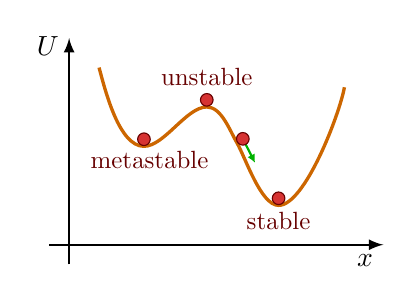
\begin{tikzpicture}
  \def\ymax{2.5}
  \def\xmax{3.8}
  \coordinate (O) at (0,0);
  \coordinate (A) at (0.10*\xmax,0.9*\ymax);
  \coordinate (B) at (0.25*\xmax,0.5*\ymax); % metastable eq.
  \coordinate (C) at (0.46*\xmax,0.7*\ymax); % instable eq.
  \coordinate (D) at (0.56*\xmax,0.52*\ymax); % no eq.
  \coordinate (E) at (0.70*\xmax,0.2*\ymax); % stable eq.
  \coordinate (F) at (0.92*\xmax,0.8*\ymax);
  \draw[->,thick] (0,-0.1*\ymax) -- (0,1.05*\ymax) node[below=3,left] {$U$}; %=mgh
  \draw[->,thick] (-0.1*\ymax,0) -- (1.05*\xmax,0) node[below left] {$x$};
  \draw[very thick,orange!80!black]
    (A) to[out=-75,in=180,looseness=0.7] (B)
        to[out=0,in=180,looseness=0.7] (C)
        to[out=0,in=120,looseness=0.8] (D)
        to[out=-60,in=180,looseness=0.6] (E)
        to[out=0,in=-100,looseness=0.5] (F);
  \draw[myarr,vcol,thick] (D)++(30:0.09) --++ (-63:0.09*\xmax);
  \draw[CM] (B)++(0,0.09) circle(0.08) node[right=2,below=1,scale=0.9] {metastable};
  \draw[CM] (C)++(0,0.09) circle(0.08) node[above=2,scale=0.9] {unstable};
  \draw[CM] (D)++(30:0.09) circle(0.08); %node[above right=0,scale=0.9] {no eq.};
  \draw[CM] (E)++(0,0.09) circle(0.08) node[below=2,scale=0.9] {stable};
  %\draw[myarr] (B)++(50:0.07*\xmax) --++ (44:0.1*\xmax);
\end{tikzpicture}


% INSTABILITY including neutral equilibrium
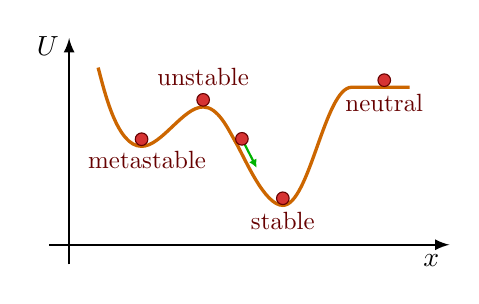
\begin{tikzpicture}
  \def\ymax{2.5}
  \def\xmax{4.6}
  \coordinate (O) at (0,0);
  \coordinate (A) at (0.08*\xmax,0.9*\ymax);
  \coordinate (B) at (0.20*\xmax,0.5*\ymax);  % metastable eq.
  \coordinate (C) at (0.37*\xmax,0.7*\ymax);  % instable eq.
  \coordinate (D) at (0.46*\xmax,0.52*\ymax); % no eq.
  \coordinate (E) at (0.59*\xmax,0.2*\ymax);  % stable eq.
  \coordinate (F) at (0.78*\xmax,0.8*\ymax);
  \coordinate (G) at (0.87*\xmax,0.8*\ymax);  % neutral eq.
  \coordinate (H) at (0.94*\xmax,0.8*\ymax);
  \draw[->,thick] (0,-0.1*\ymax) -- (0,1.05*\ymax) node[below=3,left] {$U$}; %=mgh
  \draw[->,thick] (-0.1*\ymax,0) -- (1.05*\xmax,0) node[below left] {$x$};
  \draw[very thick,orange!80!black]
    (A) to[out=-75,in=180,looseness=0.7] (B) % metastable eq.
        to[out=0,in=180,looseness=0.7] (C)   % instable eq.
        to[out=0,in=120,looseness=0.8] (D)   % no eq.
        to[out=-60,in=180,looseness=0.6] (E) % stable eq.
        to[out=0,in=180,looseness=0.5] (F)
        to[out=0,in=180,looseness=2] (G)     % neutral eq.
        to[out=0,in=180,looseness=0.5] (H);
  \draw[myarr,vcol,thick] (D)++(30:0.09) --++ (-63:0.09*\xmax);
  \draw[CM] (B)++(0,0.09) circle(0.08) node[right=2,below=1,scale=0.9] {metastable};
  \draw[CM] (C)++(0,0.09) circle(0.08) node[above=2,scale=0.9] {unstable};
  \draw[CM] (D)++(30:0.09) circle(0.08); %node[above right=0,scale=0.9] {no eq.};
  \draw[CM] (E)++(0,0.09) circle(0.08) node[below=2,scale=0.9] {stable};
  \draw[CM] (G)++(0,0.09) circle(0.08) node[below=2,scale=0.9] {neutral};
  %\draw[myarr] (B)++(50:0.07*\xmax) --++ (44:0.1*\xmax);
\end{tikzpicture}


\end{document}
